\documentclass[12pt]{article}

\usepackage{amsmath}
\usepackage{amssymb}
\usepackage{graphicx}
\usepackage{geometry}
\DeclareMathOperator{\arcsec}{arcsec}
\geometry{margin=1in}

\begin{document}

\begin{titlepage}
\centering
\vspace*{1.2in}

{\Large AP Calculus Final Project\par}

\vspace{0.9in}

{\huge\bfseries An Algebraic, Graphical, and Numerical Study of Trigonometric Substitution\par}

\vspace{0.25in}

{\Large with an Application in Physics
\par}

\vspace{1.1in}

{\large
Gordon Wang\\
David Duan\\
Sebastian Xi
\par}

\vfill

{\large \today\par}

\end{titlepage}

\section*{Abstract}
Trigonometric substitution is a technique used in calculus to evaluate integrals involving radical expressions such as \(\sqrt{a^2 - x^2}\), \(\sqrt{a^2 + x^2}\), and \(\sqrt{x^2 - a^2}\). This paper explains how the three major trigonometric substitutions work, how the domain restrictions affect the method, how the results can be interpreted graphically and numerically, and how trigonometric substitutions can be used in physics.

\section{Introduction}

In integration, many expressions are difficult to handle directly because they contain square roots of quadratic expressions, such as \(a^2 - x^2\), \(a^2 + x^2\), and \(x^2 - a^2\). These forms are related to Pythagorean identities. Therefore, using trigonometric functions to replace the variable \(x\) can provide a way to work around the radicals. For instance, if an integral contains \(\sqrt{a^2 - x^2}\), the substitution \(x = a\sin(\theta)\) can eliminate the radical because of the identity \(1 - \sin^2(\theta) = \cos^2(\theta)\).

This paper explains trigonometric substitution algebraically, graphically, and numerically. It also discusses how this technique is powerful in physics, especially in problems involving fields. The goal is to reveal the hidden properties within trigonometric substitutions.

\section{Key Cautions: Domain, Range, Sign, and Absolute Value}

Before using trigonometric substitution, it is important to understand the restrictions that come with it.

First, the original expression may have its own domain that is not simply all real numbers. For instance, \(\sqrt{a^2 - x^2}\) is only defined when \(-a \le x \le a\), assuming \(a > 0\). The expression \(\sqrt{x^2 - a^2}\) is only defined when \(x \le -a\) or \(x \ge a\).

Second, the trigonometric functions used in the substitutions must be restricted so that the substitution is one-to-one –- this allows reversing the substitution later. For instance, when using \(x = a\sin(\theta)\), it is common to choose \(-\frac{\pi}{2} \le \theta \le \frac{\pi}{2}\) because sine is one-to-one on that interval.

Third, absolute values must be handled carefully. For instance, \(\sqrt{\cos^2(\theta)} = |\cos(\theta)|\), instead of \(\sqrt{\cos^2(\theta)} = \cos(\theta)\), should be used in the intermediate steps of substitution.

The absolute values also hint at the piecewise nature of the results that this paper discusses in the later sections.

\section{Derivation of the Three Main Substitutions}

The three main trigonometric substitutions are based on the Pythagorean identities
\[
1-\sin^2\theta=\cos^2\theta,\qquad
1+\tan^2\theta=\sec^2\theta,\qquad
\sec^2\theta-1=\tan^2\theta
\]
Assume \(a>0\).

\subsection*{1. Integrals Involving \(\sqrt{a^2-u^2}\)}

For integrals involving
\[
\sqrt{a^2-u^2}
\]
let
\[
u=a\sin\theta
\]
Then
\[
\sqrt{a^2-u^2}
=\sqrt{a^2-a^2\sin^2\theta}
=\sqrt{a^2(1-\sin^2\theta)}
=\sqrt{a^2\cos^2\theta}
=a|\cos\theta|
\]
If
\[
-\frac{\pi}{2}\le \theta\le \frac{\pi}{2}
\]
then \(\cos\theta\ge 0\), so
\[
\sqrt{a^2-u^2}=a\cos\theta
\]

\begin{center}
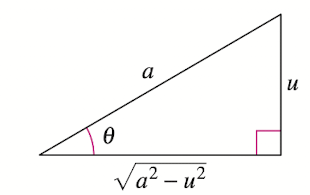
\includegraphics[width=0.45\textwidth]{figures/trig-substitution-sine.png}
\end{center}

\subsection*{2. Integrals Involving \(\sqrt{a^2+u^2}\)}

For integrals involving
\[
\sqrt{a^2+u^2}
\]
let
\[
u=a\tan\theta
\]
Then
\[
\sqrt{a^2+u^2}
=\sqrt{a^2+a^2\tan^2\theta}
=\sqrt{a^2(1+\tan^2\theta)}
=\sqrt{a^2\sec^2\theta}
=a|\sec\theta|
\]
If
\[
-\frac{\pi}{2}<\theta<\frac{\pi}{2}
\]
then \(\sec\theta>0\), so
\[
\sqrt{a^2+u^2}=a\sec\theta
\]

\begin{center}
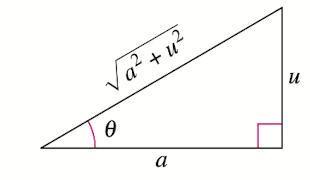
\includegraphics[width=0.45\textwidth]{figures/trig-substitution-tangent.png}
\end{center}

\subsection*{3. Integrals Involving \(\sqrt{u^2-a^2}\)}

For integrals involving
\[
\sqrt{u^2-a^2}
\]
let
\[
u=a\sec\theta
\]
Then
\[
\sqrt{u^2-a^2}
=\sqrt{a^2\sec^2\theta-a^2}
=\sqrt{a^2(\sec^2\theta-1)}
=\sqrt{a^2\tan^2\theta}
=a|\tan\theta|
\]
Therefore,
\[
\sqrt{u^2-a^2}
=
\begin{cases}
a\tan\theta, & u>a,\quad 0\le \theta\le \frac{\pi}{2}\\
-a\tan\theta, & u<-a,\quad \frac{\pi}{2}<\theta\le \pi
\end{cases}
\]

\begin{center}
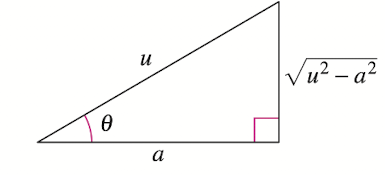
\includegraphics[width=0.45\textwidth]{figures/trig-substitution-secant.png}
\end{center}

This pair of trigonometric substitution is especially complex due to its piecewise nature. Therefore, we will present an example algebraic derivation involving this substitution in the next section of this paper.


\section{Algebraic Derivation for a Specific Example}

\[
\text{Solve } \int \frac{dx}{\sqrt{x^2 - 1}}
\]

Let
\[
\theta = \arcsec x
\]

Then
\[
x = \sec \theta
\]
where
\[
\theta \in \mathbb{R}, \qquad \theta \ne \frac{\pi}{2} + n\pi, \qquad n \in \mathbb{Z}
\]

First, consider the domain of \(x\):
\[
x^2 - 1 > 0
\]
\[
x^2 > 1
\]
\[
x > 1 \quad \text{or} \quad x < -1
\]

Note that \(x \ne \pm 1\). Thus,
\[
\sec \theta \ne \pm 1
\]

Therefore,
\[
\theta \ne 0, \pi
\]

For simplicity, we limit \(\theta\) to
\[
(0,\pi)
\]

Therefore, after considering all restrictions,
\[
\theta \in \left(0,\frac{\pi}{2}\right) \cup \left(\frac{\pi}{2},\pi\right)
\]

Since
\[
x = \sec \theta
\]
we have
\[
\frac{dx}{d\theta} = \sec \theta \tan \theta
\]

Thus,
\[
dx = \sec \theta \tan \theta \, d\theta
\]

Substituting \(dx = \sec \theta \tan \theta \, d\theta\) and \(x = \sec \theta\) into the original integral:
\[
\int \frac{dx}{\sqrt{x^2 - 1}}
=
\int \frac{\sec \theta \tan \theta \, d\theta}{\sqrt{\sec^2 \theta - 1}}
\]

Using
\[
\sec^2 \theta - 1 = \tan^2 \theta
\]
we get
\[
\int \frac{\sec \theta \tan \theta \, d\theta}{\sqrt{\tan^2 \theta}}
=
\int \frac{\sec \theta \tan \theta \, d\theta}{|\tan \theta|}
\]

This is a piecewise integral:
\[
\int \frac{\sec \theta \tan \theta \, d\theta}{|\tan \theta|}
=
\begin{cases}
\displaystyle \int \frac{\sec \theta \tan \theta}{\tan \theta} \, d\theta
& \theta \in \left(0,\frac{\pi}{2}\right) \\[1.2em]
\displaystyle \int \frac{\sec \theta \tan \theta}{-\tan \theta} \, d\theta
& \theta \in \left(\frac{\pi}{2},\pi\right)
\end{cases}
\]

Therefore,
\[
=
\begin{cases}
\displaystyle \int \sec \theta \, d\theta
& \theta \in \left(0,\frac{\pi}{2}\right) \\[1.2em]
\displaystyle \int -\sec \theta \, d\theta
& \theta \in \left(\frac{\pi}{2},\pi\right)
\end{cases}
\]

Since
\[
\int \sec \theta \, d\theta
=
\ln |\tan \theta + \sec \theta| + C
\]
we get
\[
=
\begin{cases}
\ln |\tan \theta + \sec \theta| + C_1
& \theta \in \left(0,\frac{\pi}{2}\right) \\[0.8em]
-\ln |\tan \theta + \sec \theta| + C_2
& \theta \in \left(\frac{\pi}{2},\pi\right)
\end{cases}
\]

Substitute \(\theta = \arcsec x\) back:
\[
=
\begin{cases}
\ln |\tan(\arcsec x) + \sec(\arcsec x)| + C_1
& x \in (1,\infty) \\[0.8em]
-\ln |\tan(\arcsec x) + \sec(\arcsec x)| + C_2
& x \in (-\infty,-1)
\end{cases}
\]

Now consider \(\tan(\arcsec x)\). Since
\[
\sec(\arcsec x) = x
\]
and
\[
\tan^2 \theta + 1 = \sec^2 \theta
\]
we have
\[
\tan \theta
=
\begin{cases}
\sqrt{\sec^2 \theta - 1}
& \theta \in (0,\frac{\pi}{2}) \\[0.8em]
-\sqrt{\sec^2 \theta - 1}
& \theta \in (\frac{\pi}{2},\pi)
\end{cases}
\]

Therefore,
\[
\tan(\arcsec x)
=
\begin{cases}
\sqrt{x^2 - 1}
& x \in (1,\infty) \\[0.8em]
-\sqrt{x^2 - 1}
& x \in (-\infty,-1)
\end{cases}
\]

Thus,
\[
\int \frac{dx}{\sqrt{x^2 - 1}}
=
\begin{cases}
\ln \left|x+\sqrt{x^2 - 1}\right| + C_1
& x \in (1,\infty) \\[0.8em]
-\ln \left|x-\sqrt{x^2 - 1}\right| + C_2
& x \in (-\infty,-1)
\end{cases}
\]

Using the domain restrictions to remove the absolute values, we can rewrite the final result as
\[
\boxed{
\int \frac{dx}{\sqrt{x^2 - 1}}
=
\begin{cases}
\ln \left(x+\sqrt{x^2 - 1}\right) + C_1
& x \in (1,\infty) \\[0.8em]
-\ln \left(-x+\sqrt{x^2 - 1}\right) + C_2
& x \in (-\infty,-1)
\end{cases}
}
\]


\section{Graphical Interpretation}

One caveat about the relationship between the domain of the integrand and the antiderivative is that, for an antiderivative, the domain is split wherever the integrand is discontinuous, and the antiderivative is defined separately on each interval where the integrand is continuous.

\subsection*{Graph of \(\frac{1}{\sqrt{x^2-1}}\)}

\begin{center}
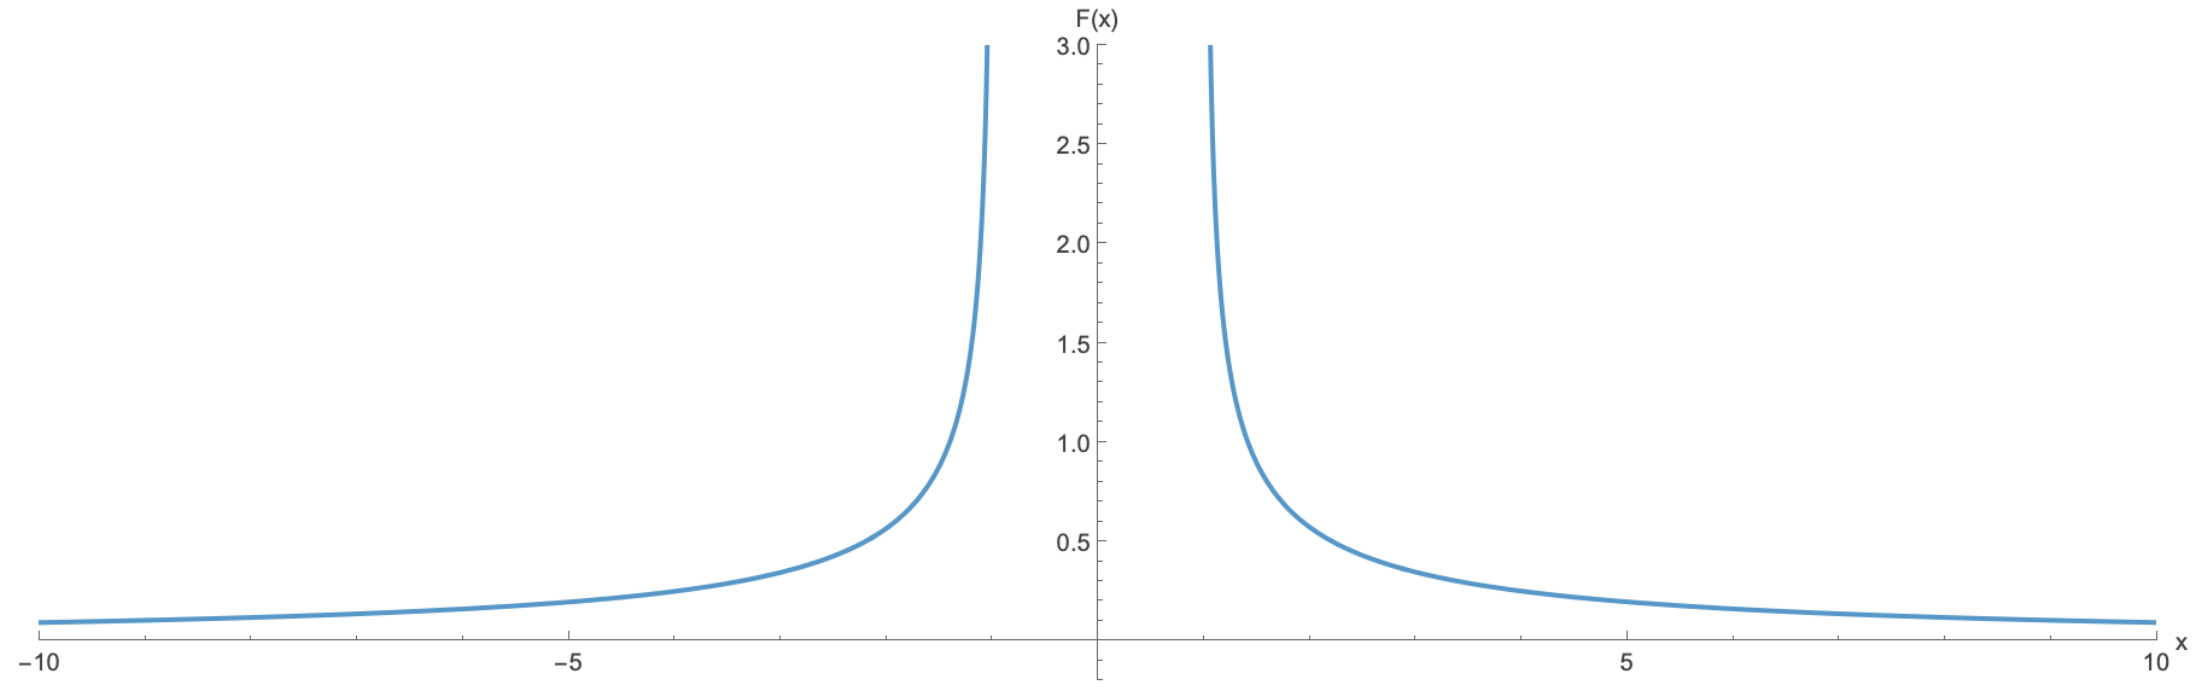
\includegraphics[width=0.9\textwidth]{figures/integrand-reciprocal-root.png}
\end{center}

This graph represents the integrand
\[
f(x)=\frac{1}{\sqrt{x^2-1}}
\]

From the graph, it is clear that it is only defined when \(x<-1\) or \(x>1\), which means it is not continuous. As mentioned previously, the antiderivative is defined separately on each interval where the integrand is continuous. This also explains the piecewise nature of the solution that is found in the previous section.

When considering the overall trend, the graph becomes very large near \(x=-1\) and \(x=1\), so an antiderivative should also have very steep slopes near those points.

\subsection*{Graph of \(\ln\left|x+\sqrt{x^2-1}\right|\)}

\begin{center}
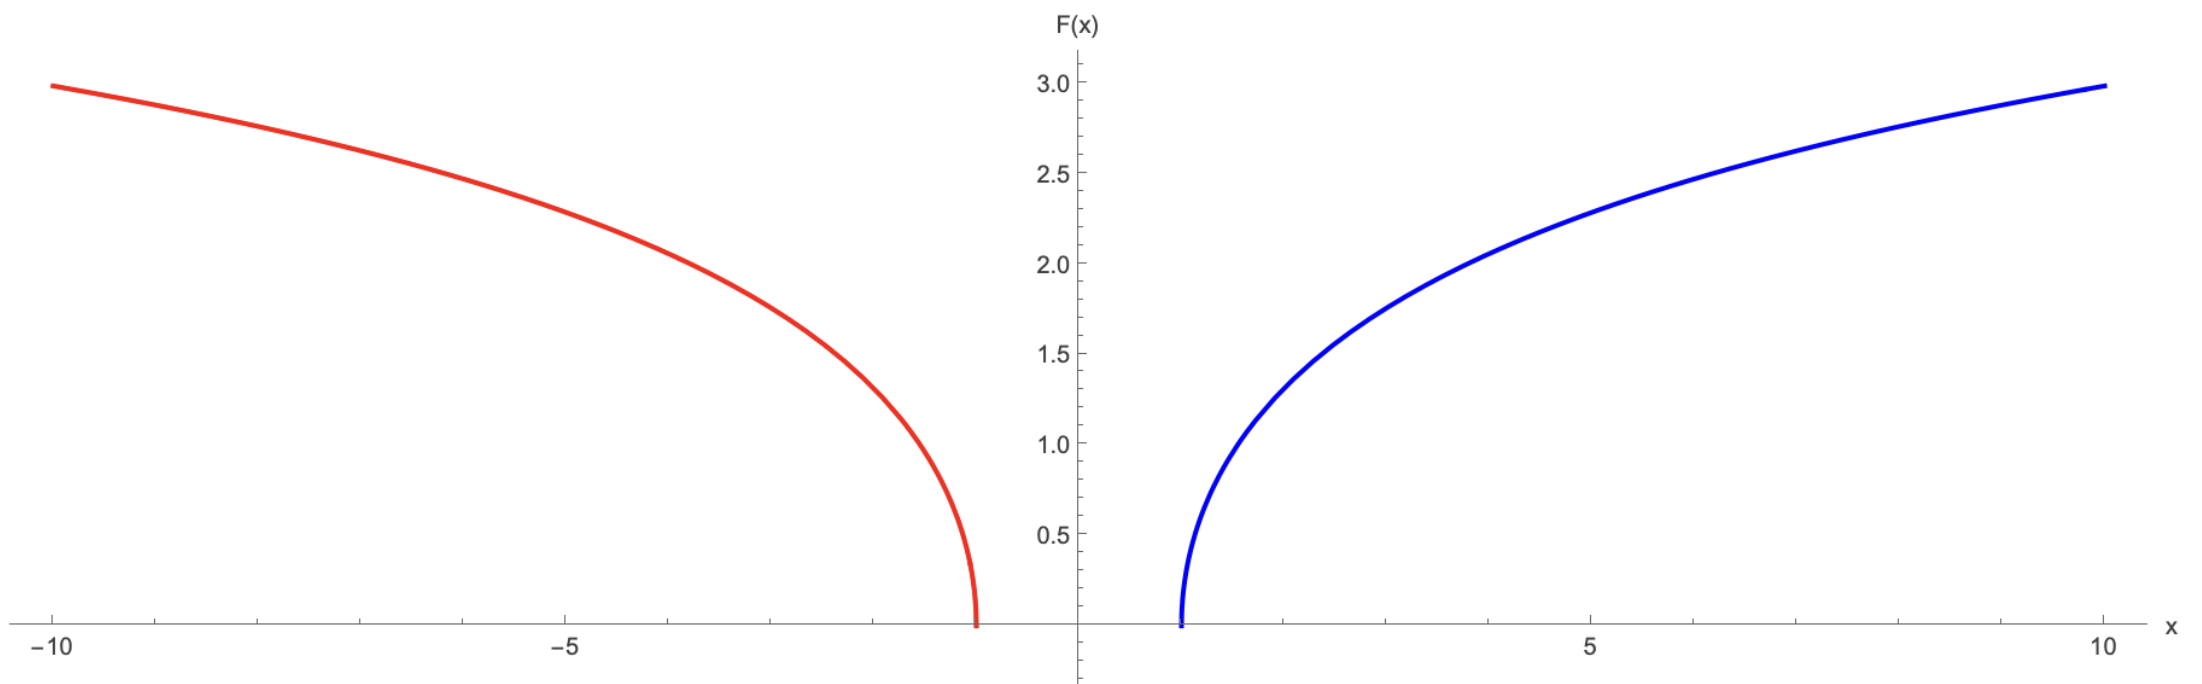
\includegraphics[width=0.9\textwidth]{figures/antiderivative-log-root.png}
\end{center}

This graph represents the antiderivative
\[
F(x)=\ln\left|x+\sqrt{x^2-1}\right|
\]
The two graphs align because at the points where \(\frac{1}{\sqrt{x^2-1}}\) is large, the graph of \(F(x)\) changes quickly; where \(\frac{1}{\sqrt{x^2-1}}\) is small, the graph of \(F(x)\) changes slowly. This matches the idea that \(F(x)\) is the integral of \(f(x)\).

\section{Numerical Evaluation with Definite Integrals}

The result from the previous section can be used to evaluate definite integrals involving
\[
\frac{1}{\sqrt{x^2-1}}
\]
Since this function is only defined for \(x<-1\) or \(x>1\), the interval of integration must be chosen carefully.

\subsection*{Normal Definite Integral}

First, consider the definite integral
\[
\int_2^3 \frac{dx}{\sqrt{x^2-1}}
\]
This is a normal definite integral because the function is continuous on the entire interval \([2,3]\). Using the antiderivative from the previous section,
\[
F(x)=\ln\left|x+\sqrt{x^2-1}\right|
\]
we get
\[
\int_2^3 \frac{dx}{\sqrt{x^2-1}}
=F(3)-F(2)
\]
Therefore,
\[
\int_2^3 \frac{dx}{\sqrt{x^2-1}}
=
\ln\left(3+\sqrt{8}\right)-\ln\left(2+\sqrt{3}\right)
\]
Using logarithm properties,
\[
\int_2^3 \frac{dx}{\sqrt{x^2-1}}
=
\ln\left(\frac{3+\sqrt{8}}{2+\sqrt{3}}\right)
\]
Numerically,
\[
\boxed{
\int_2^3 \frac{dx}{\sqrt{x^2-1}}
=
\ln\left(\frac{3+\sqrt{8}}{2+\sqrt{3}}\right)
\approx 0.4458
}
\]

\subsection*{Improper Definite Integral}

Now consider the definite integral
\[
\int_1^2 \frac{dx}{\sqrt{x^2-1}}
\]
This is an improper integral because the integrand is undefined at \(x=1\). Therefore, it must be rewritten as a limit:
\[
\int_1^2 \frac{dx}{\sqrt{x^2-1}}
=
\lim_{b\to 1^+}\int_b^2 \frac{dx}{\sqrt{x^2-1}}
\]
Using the same antiderivative,
\[
\lim_{b\to 1^+}\int_b^2 \frac{dx}{\sqrt{x^2-1}}
=
\lim_{b\to 1^+}
\left[
\ln\left(x+\sqrt{x^2-1}\right)
\right]_b^2
\]
Thus,
\[
\int_1^2 \frac{dx}{\sqrt{x^2-1}}
=
\lim_{b\to 1^+}
\left(
\ln\left(2+\sqrt{3}\right)
-
\ln\left(b+\sqrt{b^2-1}\right)
\right)
\]
Since
\[
\lim_{b\to 1^+}\ln\left(b+\sqrt{b^2-1}\right)=\ln(1)=0
\]
we get
\[
\int_1^2 \frac{dx}{\sqrt{x^2-1}}
=
\ln\left(2+\sqrt{3}\right)
\]
Numerically,
\[
\boxed{
\int_1^2 \frac{dx}{\sqrt{x^2-1}}
=
\ln\left(2+\sqrt{3}\right)
\approx 1.3170
}
\]
Even though the integrand becomes unbounded as \(x\) approaches \(1\), the improper integral converges to a finite value.

\section{Application in Physics}

One important application of trigonometric substitution in physics is when calculating the electric field produced by a straight line of charge.

Suppose a uniformly charged rod of length \(2L\) lies along the \(x\)-axis, centered at the origin. The charge density is \(\lambda\), and the goal is to find the electric field at the point \(P(0,a)\), where \(a>0\).

\begin{center}
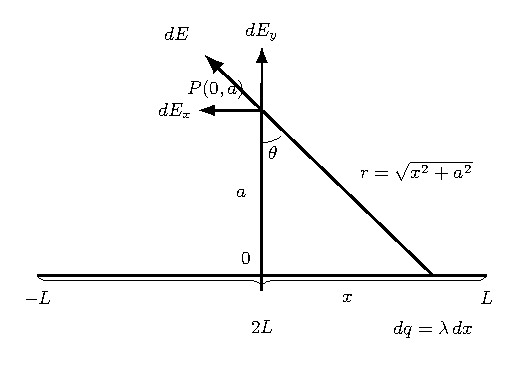
\includegraphics[width=0.75\textwidth]{figures/electric-field-line-charge.pdf}
\end{center}

For a small charge element \(dq\) located at position \(x\),
\[
dq=\lambda\,dx
\]

The distance from \(dq\) to \(P(0,a)\) is
\[
r=\sqrt{x^2+a^2}
\]

By Coulomb's law,
\[
dE=\frac{k\,dq}{r^2}
\]

Substituting \(dq=\lambda\,dx\) and \(r^2=x^2+a^2\), we get
\[
dE=\frac{k\lambda\,dx}{x^2+a^2}
\]

Only the vertical components add together. The horizontal components cancel by symmetry, so
\[
E_x=0
\]

From the right triangle,
\[
\cos\theta=\frac{a}{r}
=
\frac{a}{\sqrt{x^2+a^2}}
\]

Therefore,
\[
dE_y=dE\cos\theta
\]

So,
\[
dE_y
=
\frac{k\lambda\,dx}{x^2+a^2}
\cdot
\frac{a}{\sqrt{x^2+a^2}}
=
\frac{k\lambda a\,dx}{(x^2+a^2)^{3/2}}
\]

Thus, the total vertical electric field is
\[
E_y
=
\int_{-L}^{L}
\frac{k\lambda a\,dx}{(x^2+a^2)^{3/2}}
\]

Using the trigonometric substitution
\[
x=a\tan\theta
\]

Then
\[
dx=a\sec^2\theta\,d\theta
\]
and
\[
x^2+a^2
=
a^2\tan^2\theta+a^2
=
a^2\sec^2\theta
\]

Therefore,
\[
(x^2+a^2)^{3/2}
=
a^3\sec^3\theta
\]

The limits become
\[
x=-L \Rightarrow \theta=\tan^{-1}\left(\frac{-L}{a}\right)
\]
and
\[
x=L \Rightarrow \theta=\tan^{-1}\left(\frac{L}{a}\right)
\]

Substituting into the integral,
\[
E_y
=
\int_{\tan^{-1}(-L/a)}^{\tan^{-1}(L/a)}
\frac{k\lambda a\cdot a\sec^2\theta}{a^3\sec^3\theta}
\,d\theta
\]

Simplifying,
\[
E_y
=
\frac{k\lambda}{a}
\int_{\tan^{-1}(-L/a)}^{\tan^{-1}(L/a)}
\cos\theta\,d\theta
\]

So,
\[
E_y
=
\frac{k\lambda}{a}
\left[\sin\theta\right]_{\tan^{-1}(-L/a)}^{\tan^{-1}(L/a)}
\]

Since
\[
\sin\left(\tan^{-1}\left(\frac{L}{a}\right)\right)
=
\frac{L}{\sqrt{L^2+a^2}}
\]
and
\[
\sin\left(\tan^{-1}\left(\frac{-L}{a}\right)\right)
=
\frac{-L}{\sqrt{L^2+a^2}}
\]
we get
\[
E_y
=
\frac{k\lambda}{a}
\left(
\frac{L}{\sqrt{L^2+a^2}}
-
\frac{-L}{\sqrt{L^2+a^2}}
\right)
\]

Therefore,
\[
E_y
=
\frac{2k\lambda L}{a\sqrt{L^2+a^2}}
\]

Thus,
\[
\boxed{
E=\frac{2k\lambda L}{a\sqrt{L^2+a^2}}
}
\]
in the vertical direction. If \(\lambda>0\), the field points away from the rod; if \(\lambda<0\), it points toward the rod.

As \(L\to\infty\),
\[
\lim_{L\to\infty}
\frac{2k\lambda L}{a\sqrt{L^2+a^2}}
=
\frac{2k\lambda}{a}
\]

So, for an infinite line of charge,
\[
\boxed{
E=\frac{2k\lambda}{a}
}
\]

\section{Limitations of Trigonometric Substitutions}

Although trigonometric substitution is a powerful tool, there are limitations to it. Trigonometric substitution is most efficient when the substituted integral can be transformed using a trigonometric identity, such as the Pythagorean identities.

It is also crucial to pay careful attention to the domain, range, signs, and absolute values when solving the integral. Additionally, it is often algebraically complicated to back-substitute, which often requires using graphs to relate inverse trigonometric functions and trigonometric functions.

\section{Conclusion}

Trigonometric substitution is a powerful, yet complicated, integration technique. Algebraically, it transforms radical expressions using Pythagorean identities to simpler trigonometric functions. In physics, it appears especially powerful in problems involving fields.

By understanding trigonometric substitution algebraically and seeing it work graphically and numerically, the method reveals a much deeper meaning than just a trick to work around radicals.

\end{document}
